%\documentclass[dvipdfmx]{beamer}      % platex の場合
\documentclass[handout]{beamer}        % lualatex の場合
\usepackage{mySld}

\begin{document}
\title{基礎コンピュータ工学\\第3章 組み立て\\(パート1)}
\date{}

\begin{frame}
  \titlepage
  \centerline{\url{https://github.com/tctsigemura/TecTextBook}}
  \vfill
  \centerline{本スライドの入手:
    \raisebox{-7mm}{
\includegraphics[scale=0.3]{../Img/QRs3_1.png}}}
\end{frame}

%==============================================================================
%\begin{frame}
%  \frametitle
%  \tableofcontents
%\end{frame}

\section{組み立て}
%==============================================================================
\begin{frame}
  \frametitle{ハンダ付け}
  次のような部品から順にハンダ付けする.
  \begin{itemize}
  \item 背の低い部品
  \item 基板中心の部品
  \item 壊れにくい部品
  \end{itemize}
  \vfill
  \emph{ハンダ付け手順}\\
  \vfill
  \centerline{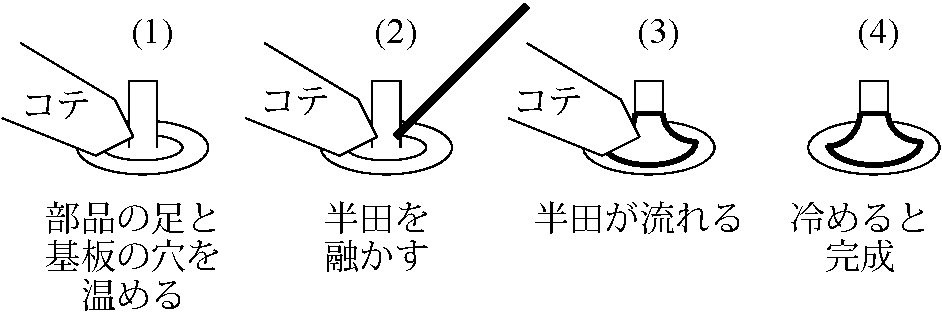
\includegraphics[scale=0.7]{../chap3/handa.pdf}}
  \vfill
\end{frame}

%==============================================================================
\begin{frame}
  \frametitle{抵抗器}
  \vfill
  \centerline{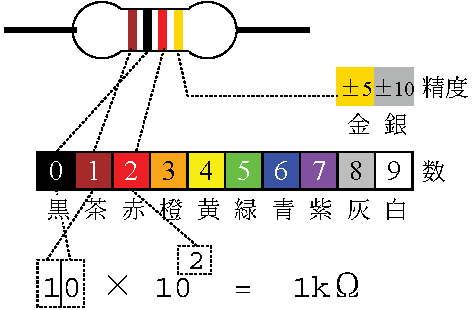
\includegraphics[scale=0.65]{../chap3/teikou.pdf}
    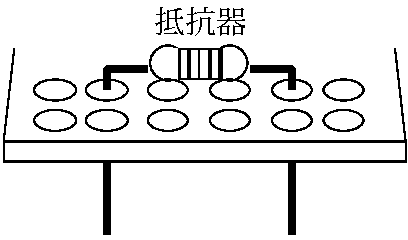
\includegraphics[scale=0.65]{../chap3/teikou2.pdf}}
  \vfill
  \centerline{\small\begin{tabular}{l|l|l}
    \hline
    \hline
    \multicolumn{1}{c|}{記号} &
    \multicolumn{1}{c|}{カラーコード} &
    \multicolumn{1}{c}{説明} \\
    \hline
    R1,15 & 黄紫茶金   & 470Ω  1/4W カーボン \\
    R7    & 茶緑黒茶茶 & 1.5kΩ 1/4W 金属皮膜 \\
    R8    & 橙黒黒茶茶 & 3.0kΩ 1/4W 金属皮膜 \\
    R9-12 & 黄紫赤金   & 4.7kΩ 1/4W カーボン \\
    R13   & 橙橙茶金   & 330Ω  1/4W カーボン \\
    R14   & 茶緑茶金   & 150Ω  1/4W カーボン \\
    R16   & 茶黒橙金   & 10kΩ  1/4W カーボン \\
  \end{tabular}}
\end{frame}

%==============================================================================
\begin{frame}
  \frametitle{積層セラミック・コンデンサ}
  \vfill
  \centerline{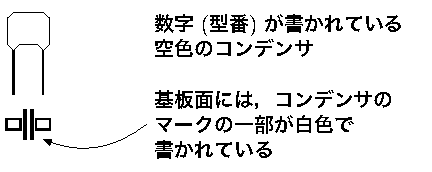
\includegraphics[scale=1.1]{../Tikz/sekisou.pdf}}
  \vfill
  \centerline{\small\begin{tabular}{l|l|l}
    \hline
    \hline
    \multicolumn{1}{c|}{記号} &
    \multicolumn{1}{c|}{型番} &
    \multicolumn{1}{c}{説明} \\
    \hline
    C1,2                &  47 & $  47 pF $    \\
    C3,4,12-15,17-34,37 & 104 & $ 0.1 \mu F $ \\
    C35                 & 101 & $ 100 pF $    \\
    C6,8,10,36          & 475 & $ 4.7 \mu F $ \\
  \end{tabular}}
  \vfill
\end{frame}

%==============================================================================
%\begin{frame}
%  \frametitle{}
%\end{frame}

\end{document}
